\chapter{Grundlagen}\label{chapter:basics}
\section{Notationen}
In dieser Arbeit werden verschiedene Notationen aus der Statistik und dem
Machine-Learning-Umfeld verwendet und sollen hier aufgrund der Les- und
Verständlichkeit aufgelistet werden.

\paragraph{Erwartungswert.}
Der Term $\mathbb{E}_{x \sim P}\left[f(x)\right]$ stellt den Erwartungswert
einer Verteilung $P$ dar und liest sich als \textit{erwarteter Wert von
$f(x)$ unter $x$ verteilt als $P$}.

\paragraph{Berechnung von Gradienten.}
Der Term $\nabla_w\left[f(x)\right]$ stellt die Berechnung der Gradienten von
den Parametern $w$ mithilfe der Loss-Funktion $f$ dar.

\section{Lipschitzstetigkeit}
\begin{definition}[K-Lipschitzstetigkeit]
Seien $(X, d_X)$ und $(Y, d_Y)$ metrische Räume. Eine Abbildung $f: X \to Y$
wird als K-lipschitzstetig bezeichnet, wenn
\[
    d_Y(f(x_1), f(x_2)) \leq K \cdot d_X(x_1, x_2)
\]
für alle $x_1, x_2 \in X$ gilt. $K$ wird hierbei als Lipschitzkonstante
bezeichnet und muss immer $K \geq 0$ erfüllen.
\end{definition}

\section{Kullback-Leibler-Divergenz}
Die Kullback-Leibler-Divergenz (KL-Divergenz) misst, wie sehr sich zwei
Verteilungen voneinander unterscheiden und hat seinen Ursprung in der
Informationstheorie. 
\begin{definition}[Kullback-Leibler-Divergenz \cite{arjovsky2017wasserstein}]
Seien $P$ und $Q$ zwei Wahrscheinlichkeitsfunktionen über den gleichen
Wahrscheinlichkeitsraum $X$. Dann ist der Abstand bzw. die Divergenz der
beiden Verteilungen definiert als
\[
    D_{KL}(P \lvert\lvert Q) = \sum_{x \in X} P(x) \log \frac{P(x)}{Q(x)}.
\]
\end{definition}
Dabei gibt $P \lvert\lvert Q$ eine Divergenz von der Ausgangsverteilung $P$
zur Zielverteilung $Q$ an. Das Messen der Divergenz zwischen zwei
Wahrscheinlichkeitsverteilungen findet insbesondere im Machine-Learning statt,
um künstliche neuronale Netze und ihre Gewichte zu trainieren. Deshalb kann
die KL-Divergenz auch als Loss-Funktion verwendet werden. Bemerkenswert ist
hierbei, dass die KL-Divergenz asymmetrisch ist, also $D_{KL}(P \lvert\lvert
Q) \neq D_{KL}(Q \lvert\lvert P)$. Die Distanz zwischen zwei Verteilungen
unterscheidet sich demnach je nach Ausgangsverteilung.

\section{Jensen-Shannon-Divergenz}
\begin{definition}[Jensen-Shannon-Divergenz \cite{arjovsky2017wasserstein}]
Seien $P$ und $Q$ zwei Wahr\-schein\-lichkeitsfunktionen über den gleichen
Wahrscheinlichkeitsraum $X$. Dann ist die Jensen-Shannon-Divergenz der
beiden Verteilungen definiert als
\[
    D_{JS}(P \lvert\lvert Q) = \frac{1}{2} D_{KL}(P \lvert\lvert M) + \frac{1}{2} D_{KL}(Q \lvert\lvert M) \quad\quad \text{mit} \;\; M = \frac{1}{2}(P + Q)
\]
\end{definition}
Die Jensen-Shannon-Divergenz kann als Erweiterung der
Kullback-Leibler-Divergenz angesehen werden. Im Gegensatz zur
Kullback-Leibler-Divergenz ist die Jensen-Shannon-Divergenz (JS-Divergenz)
symmetrisch. Das bedeutet, dass der Abstand zwischen zwei
Wahrscheinlichkeitsverteilungen gleich groß ist, egal von welchen er beiden
Distributionen aus betrachtet wird.

\section{Wasserstein-Abstand}
Eine weitere Methode zum Messen des Abstands zwischen zwei
Wahrscheinlichkeitsverteilungen ist die Berechnung des Wasserstein-Abstands.

\begin{definition}[Wasserstein-Abstand \cite{arjovsky2017wasserstein}]
Seien $P_r$ und $P_g$ zwei Wahrscheinlichkeitsverteilungen, dann ist der
Wasserstein-Abstand definiert als
\[
    W(P_r, P_g) = \inf_{\gamma \in \Pi(P_r, P_g)} \mathbb{E}_{(x, y) \sim \gamma} \left[\|x - y\|\right],
\]
wobei $\Pi(P_r, P_g)$ die Menge aller gemeinsamen Verteilungen $\gamma(x,
y)$ darstellt, dessen Grenzen $P_r$ und $P_g$ sind.
\end{definition}

Der Term $\gamma(x, y)$ stellt dabei die \textit{Masse} dar, die von $x$ nach
$y$ transportiert wird, um schließlich die Verteilung $P_r$ in die Verteilung
$P_g$ umzuformen. Aus diesem Grund ist der Wasserstein-Abstand auch als
\textit{Earth-Mover-Abstand} (EM-Abstand) bekannt.

\section{Feature-Pyramid-Networks}
Bei der Objekterkennung ist beim Erlernen der Features eines Bildes die
Auflösung dieser Features sehr gering. Feature-Pyramid-Networks (FPN) haben die
Aufgabe, eine hohe Semantik bei einer hohen Auflösung zu generieren. Häufig sind
diese Netzwerke nur Teil eines Backbones bzw. werden dahinter geschaltet. Als
Backbone-Modell kann zum Beispiel AlexNet, MobileNet und ResNet dienen. In
Kombination mit einem FPN werden diese Netze damit zu einem Feature-Extractor
umgewandelt, der eine hohe Semantik bei einer hohen Auflösung der Features
erlernen kann. Der Weg von der Eingabe über das Backbone-Modell wird auch als
\textit{Bottom-Up-Pathway} bezeichnet, während der Weg vom Backbone über die
Feature-Pyramid als \textit{Top-Down-Pathway} bezeichnet wird
\cite{lin2017feature}.

Anfänglich wurden FPNs in Verbindung mit ResNet-Backbones eingeführt (siehe
Abbildung \ref{fig:resnet-fpn}). Die Eingabe ist ein $224 \times 224 \times 3$
Bild und wird mithilfe der ersten ResNet-Schicht (C1) in $112 \times 112 \times
64$ Filter mithilfe eines Convolutional-Layers mit einem Stride von 2 und einem
$7 \times 7$ Kernel umgeformt. Anschließend wird die Ausgabe in ein
Max-Pooling-Block gegeben, welcher die Eingabe in $56 \times 56 \times 128$
Filter umwandelt. Die nächsten Blöcke sind für die Einbettung von FPNs am
wichtigsten. Der folgende Block (C2) besteht aus mehreren Residual-Blocks,
welche zusammen einen Stride von 1 ergeben und 256 Filter erzeugen. Diese Blöcke
werden zusammengefasst auch \textit{Bottlenecks} genannt. Darauf folgen drei
weitere Bottleneck-Blöcke (C3, C4, C5) mit einem Stride von 2. Nach C5 ensteht
somit eine Ausgabe von $7 \times 7 \times 2048$. Soweit zum Aufbau des
Bottom-Up-Pathways. Der Top-Down-Pathway wird mithilfe von Verbindungsschichten
(Laterals) mit dem Backbone verbunden. Diese haben die Aufgabe, die Anzahl der
Filter aus dem Bottom-Up-Pathway zu umzuformen, sodass diese im Top-Down-Pathway
miteinander addiert werden können. Hierfür werden Convolutional-Layer mit einem
$1 \times 1$ Kernel und 256 Filtern verwendet, sodass lediglich die Anzahl der
Filter transformiert werden. Im Konkreten bedeutet dies, dass die Ausgabe von C5
von $7 \times 7 \times 2048$ auf die Form $7 \times 7 \times 256$ gebracht wird.
Die Größe dieser Ausgabe wird nun mithilfe von Upsampling (M5) verdoppelt und
mit der Ausgabe der Lateralverbindung von C4 addiert (M4). Dies wird mit den übrigen Lateralverbindungen und Bottleneck-Blöcken verkettet wiederholt, sodass das FPN schließlich eine Ausgabe $56 \times 56 \times 256$ ausgibt. 

\begin{figure}
    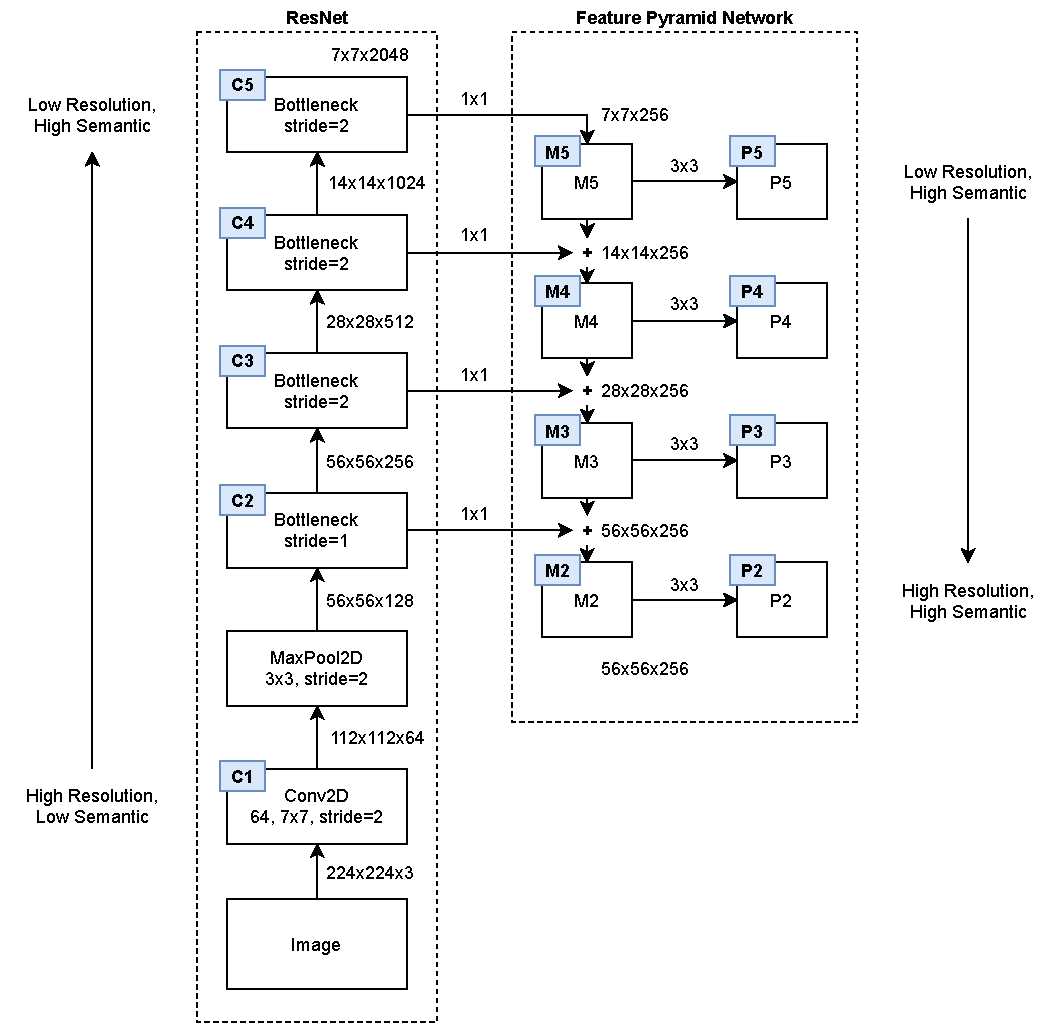
\includegraphics[width=\textwidth]{images/ResNet_FPN.pdf}
    \caption{Architektur eines Feature-Extractors als Feature-Pyramid-Network
    mit ResNet als Backbone.}
    \label{fig:resnet-fpn}
\end{figure}